\documentclass[a4paper,10pt]{article}
\usepackage[utf8]{inputenc}
\usepackage{graphicx}
\usepackage{amsmath}
\usepackage{hyperref}
\usepackage{float}
\usepackage[margin=1in]{geometry}

\title{Summary report for Machine Learning}

\author{Magdalena Pakuła \& Jakub Pawlak}

\date{\today}

\begin{document}


\maketitle

\section*{Abstract}
This project aims to design, implement and analyze the results of predicting
users' ratings on various movies using selected techniques such as: KNN, Decision Trees,
Collaborative Filtering and custom person similarity measures.
A detail overview of the methods is described with results and key findings.

\tableofcontents
\newpage

\section{KNN approach}
\subsection{Overview}
The nearest neighbor method was employed to determine the similarity
between movies based on various extracted features and user rating patterns.

The K-Nearest Neighbors (KNN) classifier operates by determining the
similarity between a target movie and previously watched movies,
then predicting the rating based on the most frequent label among
the nearest neighbors.
It evaluates the 5 closest movies to the target movie to make predictions, then
a customizable function calculates similarity between movies based on their features.
Lastly, the classifier finds the most common rating among the nearest
neighbors and returns it as the prediction.
The implementation optimizes distance computations by leveraging
NumPy operations and a partitioning technique to quickly retrieve the k-nearest
neighbors.

\paragraph{Feature Selection and Extraction}
The following features were extracted for each movie:

\begin{itemize}
    \item \textbf{Numerical Features:}
    \begin{itemize}
        \item \textit{Budget}: The movie's production budget.
        \item \textit{Popularity}: A TMDb metric representing the popularity of the movie.
        \item \textit{Release Year}: The year the movie was released.
        \item \textit{Revenue}: Total revenue generated by the movie.
        \item \textit{Runtime}: The duration of the movie in minutes.
        \item \textit{Vote Average}: The average rating given to the movie.
        \item \textit{Vote Count}: The total number of votes received.
    \end{itemize}
    \item \textbf{Categorical Features:}
    \begin{itemize}
        \item \textit{Genres}: A list of genres assigned to the movie.
        \item \textit{Cast}: The main cast of the movie.
        \item \textit{Director}: The director(s) of the movie.
    \end{itemize}
\end{itemize}

These features were chosen because they capture both objective
properties of the movies (e.g., budget, runtime) and subjective
aspects (e.g., popularity, cast, and director) that are likely to
influence user preferences.

\paragraph{Data Preprocessing}
To prepare the features for similarity calculations, the following
preprocessing steps were applied:

\begin{itemize}
    \item \textbf{Normalization:} Numerical features were normalized using a Min-Max Scaler to transform values into the range [0, 1]. This step ensures that features with larger scales (e.g., revenue) do not dominate the similarity calculations.
    \item \textbf{Categorical Feature Encoding:} For categorical features such as genres, cast, and directors, sets were constructed, and similarity was computed using the Jaccard similarity metric.
    \item \textbf{Caching:} Responses for specific movie IDs were cached to avoid redundant API queries, optimizing performance.
\end{itemize}

\paragraph{Similarity Measures}
The similarity between movies was calculated using a weighted
combination of metrics applied to different feature types:

\begin{itemize}
    \item \textbf{Numerical Features:} The cosine similarity metric was primarily used for scalar features. Other metrics, such as Manhattan and Euclidean distances, were evaluated for comparison.
    \item \textbf{Categorical Features:} Jaccard similarity was used to compare sets of genres, cast, and directors.
    \item \textbf{Rating Similarity:} Cosine similarity was computed on user rating vectors for movies, derived from the training dataset.
\end{itemize}

The total similarity was calculated as a weighted sum of these individual
components:
\[
\text{Total Similarity} = w_\text{scalar} \cdot \text{Scalar Similarity} + w_\text{genres} \cdot \text{Genres Similarity} + w_\text{cast} \cdot \text{Cast Similarity} + w_\text{directors} \cdot \text{Directors Similarity} + w_\text{ratings} \cdot \text{Ratings Similarity}
\]

where the weights $w$ were tuned to optimize performance.

\subsection{Results}
The results demonstrated that incorporating user rating similarity
significantly improved the accuracy of predictions, as it captures
shared user preferences. Also, the combination of scalar, categorical,
and rating-based similarities provided a balanced metric,
ensuring that no single feature type dominated the predictions.

The K-Nearest Neighbour (KNN) model was trained on a subset of the dataset,
using a combination of numerical and categorical features.
The optimal number of neighbors (\texttt{n\_neighbors}) was determined
through grid search, achieving the highest accuracy with \( k = 5 \).

\paragraph{Training Data:}
Performance metrics on the training dataset included:
\begin{itemize}
    \item Accuracy:
    \item Precision:
    \item Recall:
\end{itemize}

\paragraph{Validation Data:}
On the validation set, the model demonstrated consistent performance,
indicating good generalization capabilities.

The metrics achieved:
\begin{itemize}
    \item Accuracy:
    \item Precision:
    \item Recall:
\end{itemize}

\section{Decision Tree Approach}
\subsection{Overview}
The Decision Tree approach was utilized to predict user
ratings on movies.
Various features extracted from the TMDB dataset,
such as director, movie genre, runtime, and others,
were used to build the model.
The decision tree classifier constructs a hierarchical
model based on splitting the data recursively using
feature values, aiming to maximize the homogeneity
of the resulting subsets.

\subsection{Implementation Details}
The decision tree model was implemented with a maximum depth
of 5 to balance model complexity and computational efficiency.
The implementation relied on key components:

\begin{itemize}
    \item \textbf{Splitting Criterion}: Gini impurity was used to measure the quality of splits. The Gini impurity is calculated as follows:
    \begin{equation}
    \text{Gini Impurity} = 1 - \sum_{i=1}^{k} p_i^2,
    \end{equation}
    where $p_i$ is the probability of a sample belonging to class $i$.

    \item \textbf{Feature Choices}: Features were divided into scalar (e.g., runtime), categorical (e.g., language), and multivalued (e.g., cast) types. Custom choice classes were implemented to handle these distinctions.

    \item \textbf{Stopping Criteria}: Tree induction stopped either when the maximum depth was reached or when the node became pure (i.e., all samples had the same label).

    \item \textbf{Visualization}: The \texttt{graphviz} library was used to visualize the resulting decision trees, enabling better understanding and analysis of the model.
\end{itemize}

\subsection{Induction Process}
The induction process began by finding the best feature
and corresponding split threshold to minimize Gini impurity.
If the split resulted in two valid subsets, the process
recursively created child nodes for the
\textit{success} and \textit{failure} cases.
For leaf nodes, the most frequent label in the subset was
assigned as the prediction value.

An example of an induced decision tree for a specific user
is presented in Figure~\ref{fig:decision_tree}.
It demonstrates the hierarchical structure and the
decision logic based on feature thresholds and categories.

\begin{figure}[h!]
    \centering
    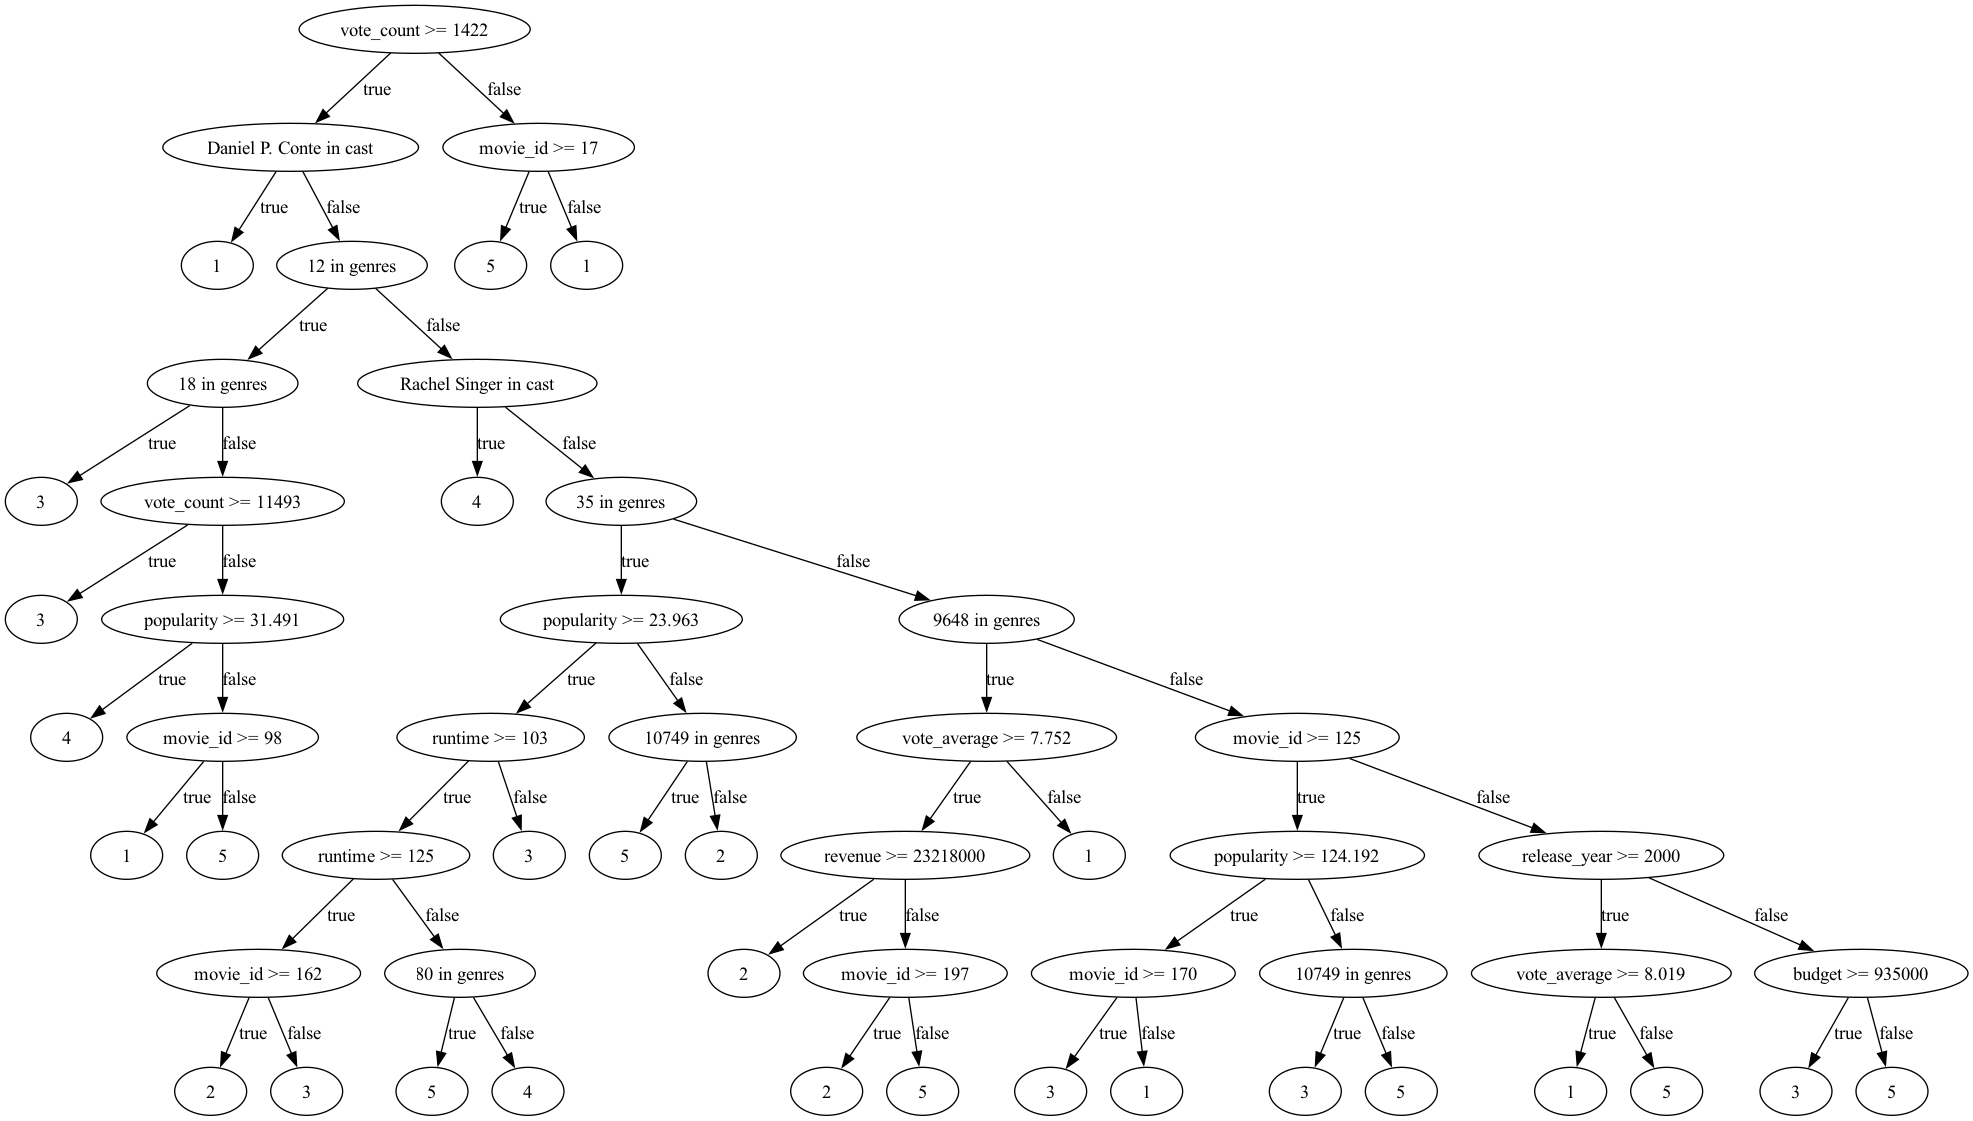
\includegraphics[width=0.8\textwidth]{tree}
    \caption{Visualization of an induced decision tree for a single user.}
    \label{fig:decision_tree}
\end{figure}

\subsection{Results}
The decision tree approach was evaluated using training and
validation datasets.
The performance metrics indicated:

\subsection{Results}
\paragraph{Training Data:}
\begin{itemize}
    \item Accuracy:
    \item Precision:
    \item Recall:
    \item Accuracy:
    \item Gini Impurity Reduction:
\end{itemize}

\paragraph{Validation Data:}
\begin{itemize}
    \item Accuracy:
    \item Precision:
    \item Recall:
    \item Accuracy:
    \item Gini Impurity Reduction:
\end{itemize}

The decision tree successfully identified patterns
in user preferences, particularly in cases where specific
features, such as genre or director, had a significant
impact on ratings.
However, the model's performance was slightly limited due
to the inherent simplicity of single decision trees and
their tendency to create hard splits.

\section{Random Forest Approach}
\subsection{Overview}
The Random Forest approach presents learning method that
combines multiple decision trees to improve predictive
performance and reduce overfitting.
Various features extracted from the TMDB dataset,
such as director, genres, runtime, and popularity,
were utilized to train the model.
The diversity of the ensemble was ensured by randomly
selecting subsets of features for each tree and using
bootstrapping to create different training datasets for
individual trees.

\paragraph{Implementation Details}
The Random Forest model was implemented with the
following key components:

\begin{itemize}
    \item \textbf{Feature Selection}: A custom class, \texttt{\_RandomFeatureSelector}, was implemented to select a random subset of features for each tree. Features such as \texttt{budget}, \texttt{genres}, \texttt{popularity}, and others were considered, while uniquely identifying features like \texttt{title} were excluded to enhance generalization.
    \item \textbf{Bootstrapping}: To create diverse training datasets for the ensemble, bootstrapped samples were generated by randomly selecting movies with replacement. Each sample included both the selected features and their corresponding ratings.
    \item \textbf{Decision Trees}: Individual decision trees were trained on the bootstrapped datasets with a maximum depth of 5, balancing computational efficiency and model complexity.
    \item \textbf{Aggregation Function}: Predictions from all trees in the forest were aggregated using the average function, ensuring a robust final prediction.
\end{itemize}

The implementation details of the core classes are as follows:
\begin{enumerate}
    \item \texttt{\_RandomFeatureSelector}: This class randomly selects a subset of features for each movie, ensuring that individual trees in the forest focus on different aspects of the data.
    \item \texttt{RandomForestClassifier}: This class orchestrates the ensemble by creating bootstrapped datasets, fitting individual trees, and aggregating predictions.
\end{enumerate}

\paragraph{Working Principles}
The Random Forest approach ensures diversity among its ensemble members by leveraging two mechanisms:
\begin{enumerate}
    \item \textbf{Random Feature Subsets}: For each tree, a random subset of features is selected, reducing correlation between the trees.
    \item \textbf{Bootstrapping}: By training each tree on a randomly sampled subset of the training data (with replacement), the trees become more diverse.
\end{enumerate}

The final prediction for a given movie is obtained by aggregating the predictions from all individual trees using an averaging function. This approach mitigates the risk of overfitting and improves the model's generalization ability.

\paragraph{Visualization}
An example of induced decision trees from the random forest ensemble for a specific user is shown in Figure~\ref{fig:random_forest_trees}. The visualization highlights the hierarchical structure of individual trees and their decision logic based on feature thresholds.

\begin{figure}[h!]
    \centering
    \includegraphics[width=0.8\textwidth]{forest_trees}
    \caption{Sample decision trees from the random forest ensemble for a single user.}
    \label{fig:random_forest_trees}
\end{figure}

\paragraph{Results}
\paragraph{Training Data:}
\begin{itemize}
    \item Accuracy: 
    \item Precision: 
    \item Recall: 
    \item RMSE:
\end{itemize}

\paragraph{Validation Data:}
\begin{itemize}
    \item Accuracy: 
    \item Precision: 
    \item Recall:
    \item RMSE: 
\end{itemize}

The Random Forest model demonstrated strong predictive
, effectively capturing complex patterns in the data.
It outperformed the single decision tree approach by
leveraging ensemble diversity and reducing the variance
of predictions.

\section{Person Similarity Approach}
\subsection{Overview}
The Person Similarity approach was employed to predict user ratings on movies by utilizing the similarity between users based on their historical ratings. The task was to predict a target user's movie rating by identifying the best-matching users, i.e., those who rated the same movies similarly. The approach uses a combination of Pearson correlation and Cosine similarity to assess how similar two users are in terms of their movie preferences, with adjustments to handle common ratings between users.

\paragraph{Implementation Details}
The Person Similarity approach was implemented by calculating a similarity score between two users using the following key components:

\begin{itemize}
    \item \textbf{Similarity Function}: The similarity score is computed by combining Pearson correlation and Cosine similarity for the movies that both users have rated. The Pearson correlation measures the linear relationship between the two users' ratings, while Cosine similarity measures the angular distance between the rating vectors. Both metrics are normalized to ensure comparability.

    \item \textbf{Weighting Factor}: A weighting factor (\texttt{pearson\_weight}) is used to control the influence of Pearson similarity in the final combined score. A higher weight gives more importance to Pearson correlation, whereas a lower weight favors Cosine similarity.

    \item \textbf{Damping Factor}: A damping factor is applied to the final similarity score to reduce the influence of users with fewer common ratings. This helps prevent situations where a user with very few shared ratings contributes excessively to the prediction.

    \item \textbf{Similarity Caching}: To enhance computational efficiency, a cache (\texttt{similarity\_cache}) is maintained to store previously computed similarity scores between user pairs. This ensures that the similarity between two users is computed only once.
\end{itemize}

The implementation of the similarity calculation is encapsulated in the \texttt{similarity\_function}, which uses the following formula:

\begin{equation}
    \text{Pearson Similarity} = \frac{\sum_{i} (x_i - \bar{x})(y_i - \bar{y})}{\sqrt{\sum_{i} (x_i - \bar{x})^2 \sum_{i} (y_i - \bar{y})^2}},
\end{equation}
where \( x_i \) and \( y_i \) are the ratings of the two users, and \( \bar{x} \) and \( \bar{y} \) are the mean ratings for each user.

Cosine similarity is computed as:

\begin{equation}
    \text{Cosine Similarity} = \frac{\sum_{i} x_i y_i}{\sqrt{\sum_{i} x_i^2} \sqrt{\sum_{i} y_i^2}},
\end{equation}
where \( x_i \) and \( y_i \) are the ratings of the two users for the common items.

The final similarity score is the weighted average of these two metrics:

\begin{equation}
    \text{Combined Similarity} = \text{pearson\_weight} \times \text{Pearson Similarity} + (1 - \text{pearson\_weight}) \times \text{Cosine Similarity}.
\end{equation}

\paragraph{Induction Process}
The induction process begins by computing the similarity between the target user and all other users who have rated the same movie. The ratings for the target movie are weighted by the similarity score between the target user and other users. This results in a weighted sum of ratings for the target movie, which is then normalized by the sum of absolute similarities.

The predicted rating for a user on a movie is calculated as follows:

\begin{equation}
    \hat{r}_{u,m} = \frac{\sum_{v \in N(m)} sim(u,v) \cdot r_{v,m}}{\sum_{v \in N(m)} |sim(u,v)|},
\end{equation}
where \( \hat{r}_{u,m} \) is the predicted rating for user \( u \) on movie \( m \), \( sim(u,v) \) is the similarity between user \( u \) and user \( v \), and \( r_{v,m} \) is the rating given by user \( v \) to movie \( m \). \( N(m) \) denotes the set of users who have rated movie \( m \).

\subsection{Results}
\paragraph{Training Data:}
\begin{itemize}
    \item Accuracy:
    \item Precision:
    \item Recall:
    \item MSE:
    \item RMSE:
\end{itemize}

\paragraph{Validation Data:}
\begin{itemize}
    \item Accuracy:
    \item Precision:
    \item Recall:
    \item MSE:
    \item RMSE:
\end{itemize}

The Person Similarity approach demonstrated a strong ability to predict user ratings, particularly in scenarios where users had rated a substantial number of common movies. However, its performance was more limited when the overlap of rated movies was small, as the approach relies heavily on the availability of common ratings for comparison.

In conclusion, while the Person Similarity approach provides an effective method for movie rating prediction based on user similarities, its performance can be impacted by the sparsity of the rating matrix. Nonetheless, it remains a valuable technique for collaborative filtering in recommender systems.

\section{Collaborative Filtering Approach}
- Training Process: [Explain the training process and dimensionality selection].
- Generalization Methods: [Describe methods used to ensure generalization].
\subsection{Overview}
\subsection{Results}
- Training Data: [Metrics and analysis].
- Validation Data: [Metrics and discussion].

\section{Summary and Comparison}
- Summarize the results for all approaches using test data or feedback.
- Compare performance metrics and discuss the strengths and weaknesses of each method.
- [Include a table or graph for comparison, if applicable].

\section*{References}
[List any references or sources used in the preparation of the report].

\end{document}